\documentclass{article}\usepackage[]{graphicx}\usepackage[]{color}
% maxwidth is the original width if it is less than linewidth
% otherwise use linewidth (to make sure the graphics do not exceed the margin)
\makeatletter
\def\maxwidth{ %
  \ifdim\Gin@nat@width>\linewidth
    \linewidth
  \else
    \Gin@nat@width
  \fi
}
\makeatother

\definecolor{fgcolor}{rgb}{0.345, 0.345, 0.345}
\newcommand{\hlnum}[1]{\textcolor[rgb]{0.686,0.059,0.569}{#1}}%
\newcommand{\hlstr}[1]{\textcolor[rgb]{0.192,0.494,0.8}{#1}}%
\newcommand{\hlcom}[1]{\textcolor[rgb]{0.678,0.584,0.686}{\textit{#1}}}%
\newcommand{\hlopt}[1]{\textcolor[rgb]{0,0,0}{#1}}%
\newcommand{\hlstd}[1]{\textcolor[rgb]{0.345,0.345,0.345}{#1}}%
\newcommand{\hlkwa}[1]{\textcolor[rgb]{0.161,0.373,0.58}{\textbf{#1}}}%
\newcommand{\hlkwb}[1]{\textcolor[rgb]{0.69,0.353,0.396}{#1}}%
\newcommand{\hlkwc}[1]{\textcolor[rgb]{0.333,0.667,0.333}{#1}}%
\newcommand{\hlkwd}[1]{\textcolor[rgb]{0.737,0.353,0.396}{\textbf{#1}}}%
\let\hlipl\hlkwb

\usepackage{framed}
\makeatletter
\newenvironment{kframe}{%
 \def\at@end@of@kframe{}%
 \ifinner\ifhmode%
  \def\at@end@of@kframe{\end{minipage}}%
  \begin{minipage}{\columnwidth}%
 \fi\fi%
 \def\FrameCommand##1{\hskip\@totalleftmargin \hskip-\fboxsep
 \colorbox{shadecolor}{##1}\hskip-\fboxsep
     % There is no \\@totalrightmargin, so:
     \hskip-\linewidth \hskip-\@totalleftmargin \hskip\columnwidth}%
 \MakeFramed {\advance\hsize-\width
   \@totalleftmargin\z@ \linewidth\hsize
   \@setminipage}}%
 {\par\unskip\endMakeFramed%
 \at@end@of@kframe}
\makeatother

\definecolor{shadecolor}{rgb}{.97, .97, .97}
\definecolor{messagecolor}{rgb}{0, 0, 0}
\definecolor{warningcolor}{rgb}{1, 0, 1}
\definecolor{errorcolor}{rgb}{1, 0, 0}
\newenvironment{knitrout}{}{} % an empty environment to be redefined in TeX

\usepackage{alltt}
\usepackage{Sweave}
\usepackage{float}
\usepackage{graphicx}
\usepackage{tabularx}
\usepackage{siunitx}
\usepackage{amssymb} % for math symbols
\usepackage{amsmath} % for aligning equations
\usepackage{textcomp}
\usepackage{mdframed}
\usepackage[hyphens]{url}
\usepackage[small]{caption}
\setlength{\captionmargin}{30pt}
\setlength{\abovecaptionskip}{0pt}
\setlength{\belowcaptionskip}{10pt}
\topmargin -1.5cm        
\oddsidemargin -0.04cm   
\evensidemargin -0.04cm
\textwidth 16.59cm
\textheight 21.94cm 
%\pagestyle{empty} %comment if want page numbers
\parskip 7.2pt
\renewcommand{\baselinestretch}{2}
\parindent 0pt
\usepackage{lineno}
\linenumbers
\usepackage{natbib}
\bibliographystyle{..//references/styles/gcb.bst}

%cross referencing:
\usepackage{xr}
\usepackage{xr-hyper}
\externaldocument{chillfrz_supp}

\newmdenv[
  topline=true,
  bottomline=true,
  skipabove=\topsep,
  skipbelow=\topsep
]{siderules}
\IfFileExists{upquote.sty}{\usepackage{upquote}}{}
\begin{document}

\noindent \textbf{\Large{False springs coupled with warming winters alter temperate tree growth}}
%\noindent \textbf{\Large{False spring treatments coupled with warming winters alter temperate tree growth}}


\noindent Authors:\\
C. J. Chamberlain $^{1,2}$ \& E. M. Wolkovich $^{1,2,3}$
\vspace{2ex}\\
\emph{Author affiliations:}\\
$^{1}$Arnold Arboretum of Harvard University, 1300 Centre Street, Boston, Massachusetts, USA 02131; \\
$^{2}$Organismic \& Evolutionary Biology, Harvard University, 26 Oxford Street, Cambridge, Massachusetts, USA 02138; \\
$^{3}$Forest \& Conservation Sciences, Faculty of Forestry, University of British Columbia, 2424 Main Mall, Vancouver, BC V6T 1Z4\\
\vspace{2ex}
$^*$Corresponding author: 248.953.0189; cchamberlain@g.harvard.edu\\

\renewcommand{\thetable}{\arabic{table}}
\renewcommand{\thefigure}{\arabic{figure}}
\renewcommand{\labelitemi}{$-$}
\setkeys{Gin}{width=0.8\textwidth}

%%%%%%%%%%%%%%%%%%%%%%%%%%%%%%%%%%%%%%%%%%%%%%%
%%%%%%%%%%%%%%%%%%%%%%%%%%%%%%%%%%%%%%%%%%%%%%%

\section*{Abstract} %% Word limit is 350, I have 300 words now.
%% Using typically four simple, factual, numbered statements, it should:
%%  1) give the conceptual context
%%  2) state the methodological approach
%%  3) report the main results and conclusions
%%  4) include a final point headed ‘Synthesis’, which sums up the paper’s key message in generic terms that can be understood by non-specialists, indicating clearly how this study has advanced ecological understanding. ... 

\begin{enumerate}
\item  With warming temperatures, spring phenology (i.e., budburst and leafout) is advancing. Late spring freezes, however, may not advance at the same rate, leading to an increase in freezes that occur after trees initiate budburst---known as false springs---with continued warming. Through shifts in false springs, climate change may reshape forest plant communities, impacting the species and ecosystem services those communities support. Predicting false spring effects requires understanding both how warming shifts spring phenology and how false springs impact plant performance. While generally spring warming advances budburst, increasing research suggests warming winters may delay budburst through reduced chilling, which may also cause plants to leaf out slower or incompletely, decreasing spring freeze tolerance and potentially lead to higher damage from false spring events. 
\item Here, we assessed the effects of over-winter chilling (generally associated with warming winters) and false spring events on sapling phenology, growth and tissue traits, across eight temperate tree and shrub species in a lab experiment. 
\item We found that false springs slowed subsequent budburst and leafout---extending the period of greatest risk for freeze damage---and increased damage to the shoot apical meristem, decreased leaf toughness and leaf thickness. Longer chilling accelerated budburst and leafout, even under false spring conditions. Thus chilling compensated for the adverse effects of false springs on phenology. Despite the effects of false springs and chilling on phenology, we did not see any major re-ordering in the sequence of species leafout. Our results suggest climate change will reshape forest communities not through temporal reassembly, but rather through impacts on growth and leaf traits from the coupled effects of false springs with decreases in over-winter chilling under future climate change. 

\item \textbf{Synthesis:} With climate change and warming temperatures, over-winter chilling is anticipated to decrease and false springs are predicted to increase in certain regions. We found that false springs and reduced chilling both impact sapling phenology, growth and tissue traits across eight common forest tree species. This suggests that the combination of increased false springs and warmer winters could be especially detrimental to forest communities, ultimately affecting important processes such as carbon storage and nutrient cycling. % Alt ending sentence: Thus, the combination of warming across the winter (through reduced chilling) and spring (through increased false springs) could impact plant performance, survival and shape species distributions in the future, ultimately affecting important processes such as carbon uptake and nutrient cycling. 
\end{enumerate}

\vspace{2ex}
\textit{Keywords:} false spring, climate change, phenology, spring freeze, forest recruitment, temporal reassembly, budburst, temperate

\section*{Introduction}
The timing of spring in temperate deciduous forests shapes plant and animal communities and influences ecosystem services from agriculture to forest management. With warming temperatures, spring phenology (i.e., budburst and leafout, which are strongly cued by temperature) is advancing, causing longer growing seasons \citep{Chuine2001} and reshaping ecosystem dynamics. In one major example, advancing spring phenology has led to increased carbon uptake across temperate forests, which are essential carbon sinks that combat the negative effects of climate change \citep{Keenan2014}. But climate change could diminish or reverse these positive effects on carbon storage: specifically through cold snaps during the spring and warming temperatures in the winter.
  
While climate change has warmed the Northern Hemisphere, cold snaps and freezing events are still occurring. These weather events can have major impacts on plant development each spring. One such event is known as a `false spring', often defined as when temperatures drop below freezing \citep[][i.e., below -2.2$^{\circ}$C]{Schwartz2002} after budburst has initiated. Damage from false spring events can have cascading effects within a forest, from changes to nutrient cycling and carbon uptake to shifts in seedling recruitment \citep{Hufkens2012, Klosterman2018, Richardson2013}. Furthermore, false springs can increase the probability of additional freezes within a growing season by extending the period in which plants are most at risk---the time between budburst and leafout, what we refer to as the `duration of vegetative risk'. This may result in a positive feedback loop: observational studies suggest plants take longer to re-flush leaves after a false spring---up to 38 days \citep{Augspurger2009, Augspurger2013, Gu2008, Menzel2015}---which could lead to additional false springs in a season \citep{Augspurger2009}. As false springs are predicted to increase in certain regions with increased climate change \citep{Ault2015, Liu2018, Zohner2020} understanding their impacts is essential for robust forest management strategies and climate forecasting \citep{OBrien2019}. 
  
Warmer winters may also play a critical role in the future of forests as they directly impact one of the  major cues plants use to time budburst: over-winter cold temperatures (chilling), in addition to warming spring temperatures (forcing) and longer daylengths \citep{Chuine2016}. Many temperate plant species have evolved chilling requirements to avoid leafout during warm snaps in the middle of the winter, but with climate change, chilling requirements may not be met. If chilling is not met, plants may leaf out much slower or incompletely, which can in turn affect freeze tolerance. Thus, predicting climate change impacts on false springs may also require understanding the interplay of warming winters and false spring risk in forest tree species. 
  
Understanding how winter chilling and false springs may affect future forests requires knowing whether this interaction varies across species within a community. This is especially true if species have evolved along a trade-off of risking spring freezes for early access to resources. While a single-species perspective may predict all individuals to require high levels of chilling to delay budburst and ultimately diminish false spring risk, competition between species for nutrients, water and light resources in the early spring likely pushes some species---and some individuals within species---to leafout earlier \citep{Augspurger2013}. Young trees and understory species generally initiate budburst before canopy trees to benefit from higher light levels \citep {Augspurger2008, Vitasse2013}, which potentially puts these species and individuals at higher risk of freeze damage \citep{Vitasse2014}. Thus, successful forest recruitment requires seedlings and saplings to minimize false spring risk while maximizing growth. 
 
The combination of species- and lifestage-level differences in response to false springs, chilling and climate change could reshape the temporal assembly of forest communities. Species typically leafout in a similar sequence, with understory species leafing out earlier and higher canopy trees leafing out last but many studies are predicting substantial shifts in chronological order and reassembly of species' leafout with climate change \citep{Roberts2015, Laube2014}. As warming increases winter temperatures and false spring prevalence, phenological cues and their interactions are anticipated to also change, which could alter competition and recruitment among forest species for early-season resources and ultimately impact species diversity and carbon uptake in temperate forests.
  
Here, we assessed the effects of over-winter chilling length and false springs on sapling phenology and growth across eight temperate tree and shrub species. We exposed individuals to different levels of over-winter chilling crossed with a false spring event in growth chambers, then followed individuals for a growing season to understand: (1) How does over-winter chilling impact phenology, growth and physical leaf traits, (2) how do false spring events impact phenology, growth and physical leaf traits, and (3) how does the interaction between chilling and false springs impact community structure and phenological order?

\section*{Materials and Methods} 
\subsection*{Plant Selection and Material}
We selected eight temperate woody plant tree and shrub species that span varying spring phenologies (e.g., early to later leafout), that are not generally used as crops or ornamental species: \textit{Acer saccharinum}, \textit{Alnus incana rugosa}, \textit{Betula papyrifera}, \textit{Betula populifolia}, \textit{Cornus racemosa}, \textit{Salix purpurea}, \textit{Sorbus americana}, and \textit{Viburnum dentatum} (we originally included two additional species---\textit{Fagus grandifolia} and \textit{Nyssa sylvatica}, but the plants were not delivered in a usable condition and thus we excluded them from the experiment). We used 48 dormant, one year old, bare root saplings---each measuring 6-12 inches---for each species from Cold Stream Farm LLC (Freesoil, MI; 44$^{\circ}$6' N -86$^{\circ}$12' W) for a total of 384 individuals. Upon receipt---on 21 November 2018, plants were potted in 656 ml deepots with Fafard \#3B Metro Mix soil and placed in growth chambers at the Weld Hill Research Building of the Arnold Arboretum (Boston, MA; 42$^{\circ}$17' N -71$^{\circ}$8' W) at 4$^{\circ}$C for different durations depending on chilling treatment (explained below).   

\subsection*{Growth Chamber and Greenhouse Conditions}
Individuals were randomly selected for one of six experimental treatments from a full factorial design of false spring (two levels: presence or absence of false spring) x chilling (three levels: four, six or eight weeks of chilling at 4$^{\circ}$C with eight hour photoperiod, lighting was a combination of T5HO fluorescent lamps with halogen incandescent bulbs at roughly 250 $\mu mol/m^{2}/s$). Individuals were rotated within and among growth chambers every two weeks to minimize bias from possible growth chamber effects.

Once each chilling treatment was completed, we moved individuals to a greenhouse with mean daytime temperature of 15$^{\circ}$C and a mean nighttime temperature of 10$^{\circ}$C, and a photoperiod of 12 hour days throughout the spring until all individuals reached full leaf expansion. After all individuals of all species reached full leaf expansion, greenhouse temperatures and photoperiods were kept ambient, and all individuals were up-potted to 983 ml deepots and fertilized with SCOTTS 15-9-12 Osmocote Plus 5-6. 

\subsection*{Phenology and False Spring Treatment} 
We recorded phenology \citep[using the BBCH scale,][]{Meier2001} every 2-3 days through full leaf expansion. Budburst was denoted as BBCH stage 07, which is `beginning of sprouting or bud breaking' and monitored until full leaf expansion (BBCH stage 19) in order to evaluate the duration of vegetative risk \citep{Chamberlain2019} for each individual \citep{Finn2007}. Individuals in the `false spring' treatment were placed in a growth chamber set to mimic a false spring event during budburst, defined as once at least 50\% of the buds were at BBCH stage 07 but the individual had not yet reached BBCH stage 19 (that is, each sapling was exposed to a false spring based on its individual phenological timing). False spring treatments lasted approximately 14 hours, beginning at 18:00; temperatures were ramped down (Figure \ref{fig:gccond}). At approximately 08:00 the following day, we placed false spring individuals back in the greenhouse. Once all individuals reached full leaf expansion (BBCH stage 19), we recorded phenology weekly until 1 August 2019, then every 2-3 days again to monitor fall phenology. We monitored all individuals until complete budset. % 1 August ... What year?

\subsection*{Growth measurements}
We measured shoot growth as a metric of plant height three times throughout the growing season: the day an individual reached full leaf expansion, 60 days after full leaf out and when an individual reached complete budset. We measured the chlorophyll content of four leaves on each individual 60 days after full leaf out using an atLEAF CHL PLUS Chlorophyll meter, converting chlorophyll content to mg/cm\textsuperscript{2} using the atLEAF CHL PLUS conversion tool. We measured leaf thickness using a Shars Digital Micrometer (accurate to 0.001mm) and leaf toughness in Newtons using a Shimpo Digital Force Gauge on two leaves for each individual 60 days after full leaf out. Additionally, we visually monitored damage to the shoot apical meristem, which consisted of complete damage or disruption of growth in the main stem and resulted in early dormancy induction or reliance on lateral shoot growth. Finally, we harvested each plant after it reached complete budset to dry, separate and weigh belowground and aboveground biomass (including leaves). 

\subsection*{Data analysis} 
We used Bayesian hierarchical models \citep[with the brms package,][,version 2.3.1]{brms} in R \citep[][,version 3.3.1]{R} to estimate the effects of chilling duration, false spring treatment and all two-way interactions as predictors on: (1) duration of vegetative risk, (2) growing season length, (3) shoot apical meristem damage, (4) total growth in centimeters, (5) total biomass, (6) chlorophyll content, (7) leaf toughness and (8) leaf thickness. We modeled species hierarchically as grouping factors, which generated an estimate and posterior distribution for each species as well as an overall response across the eight species used in our experiment. We ran four chains, each with 4 000 iterations, of which 2 500 were warm-up iterations, for a total of 6 000 posterior samples for each predictor for each model using weakly informative priors (increasing priors three-fold did not impact our results). We evaluated our model performance based on $\hat{R}$ values that were close to 1.0, checked chain convergence and posterior predictive checks visually \citep{BDA}, and made sure all models had 0 divergent transitions. Our models generally had high $n_{eff}$ (6 000 for most parameters, but as low as 1 400 for a couple of parameters in the shoot apical meristem model). All estimated values are reported in the text as means +/- standard errors relative to the no false spring under eight weeks of chilling treatment.


\section*{Results} 
Chilling durations impacted individual phenology. As seen in many other studies, we found decreases in chilling delayed day of budburst by 4.8 $\pm$ 1.8 days for six weeks of chilling and by 7.6 $\pm$ 1.8 days for four weeks of chilling (as mentioned above, all values are given relative to the no false spring under eight weeks of chilling treatment; Table \ref{tab:simpbb}). Shorter chilling also slowed the rate of leafout, increasing the duration of vegetative risk (4 weeks: 2.7 $\pm$ 1.6 days; Figure \ref{fig:muphen}\textbf{a}, Table \ref{tab:simpdvr} and Table \ref{tab:suppmoddvr}). Decreased chilling lengthened the growing season for individuals exposed to four weeks of chilling (13.3 $\pm$ 5.1 days; Figure \ref{fig:muphen}\textbf{b} and Table \ref{tab:suppmodgs}), due to constraints on our experimental design: individuals in longer chilling treatments were put in the greenhouse two to four weeks later than the four weeks of chilling group but all individuals experienced the same ambient late summer conditions when in the greenhouse, including shifts in temperature and light associated in the late summer/autumn that generally trigger dormancy onset; thus shortening the growing season for the groups that experienced longer chilling.
 
False springs also impacted individual phenology. Individuals exposed to the false spring treatment had longer durations of vegetative risk given four weeks of chilling (5.7 $\pm$ 1.2 days) and slightly longer durations given six weeks of chilling (4.2 $\pm$ 1.1 days; Figure \ref{fig:muphen}\textbf{a} and Table \ref{tab:suppmoddvr}). Effects on the duration of vegetative risk from false spring treatments (which led to longer durations) and from increased chilling (which led to shorter durations) were generally additive, resulting in no major changes in the durations of vegetative risk for individuals exposed to a false spring that received eight weeks of chilling (3.6 $\pm$ 0.8 days, Figure \ref{fig:muphen}\textbf{a} and Table \ref{tab:suppmoddvr}). 

False springs impacted growth habit and shoot growth but not total biomass. Across all chilling treatments, especially for the eight and four week chilling treatments, false springs led to more damage to the shoot apical meristem (8 weeks: 50.0\% increase in probability of damage under false spring treatment or 2.0 $\pm$ 0.8; 6 weeks: 37.5\% or a 1.5 $\pm$ 1.3; and 4 weeks: 50.0\% or a 2.0 $\pm$ 1.4; Figure \ref{fig:mugrowth}\textbf{a} and Table \ref{tab:suppmodmeri}). Shoot growth over the growing season decreased with eight weeks of chilling under false spring conditions (-5.7 $\pm$ 4.6 cm) and shoot growth also decreased with shorter chilling durations (6 weeks: -10.7 $\pm$ 7.1 cm; 4 weeks: -6.4 $\pm$ 6.8 cm; Figure \ref{fig:mugrowth}\textbf{b} and Table \ref{tab:suppmodht}). There was very little change in total biomass under false spring conditions (compared to the no false spring) for both the six (-4.9 $\pm$ 4.1 g) and the eight weeks of chilling treatments (-6.0 $\pm$ 3.0 g; Figure \ref{fig:mutotbio} and Table \ref{tab:suppmodtotbio}) but false springs led to slightly lower total biomasses when saplings were exposed to only four weeks of chilling (-6.0 $\pm$ 3.8 g).
  
False springs also affected physical leaf traits. False spring treatments decreased leaf toughness across all chilling treatments (8 weeks: -0.03 $\pm$ 0.02 N; 6 weeks: -0.03 $\pm$ 0.02 N; and 4 weeks: 0.004 $\pm$ 0.03 N; Figure \ref{fig:muleaf}\textbf{a} and Table \ref{tab:suppmodtough}) and decreased chlorophyll content in leaves with eight and six weeks of chilling (8 weeks: -2.5 $\pm$ 0.8 mg/cm\textsuperscript{2}; and 6 weeks: -1.9 $\pm$ 1.2 mg/cm\textsuperscript{2}; Figure \ref{fig:muchl} and Table \ref{tab:suppmodchl}). Additionally, false springs led to decreased leaf thickness across eight and four weeks of chilling treatments, but there was little change for the six weeks of chilling treatment (8 weeks: -7.4 $\pm$ 3.9 $\mu$m; 6 weeks: 4.9 $\pm$ 5.5 $\mu$m; and 4 weeks: -0.7 $\pm$ 5.5 $\mu$m for eight weeks of chilling; Figure \ref{fig:muleaf}\textbf{b} and Table \ref{tab:suppmodthick}). 
  
False springs and chilling treatments were generally consistent across species, though not always. Duration of vegetative risk decreased for most species with longer chilling (i.e., the eight weeks), except for \textit{Salix purpurea}, which experienced longer durations of vegetative risk with longer chilling (Figure \ref{fig:muphen}\textbf{a}). False springs led to meristem damage across all species except for \textit{Betula populifolia} and \textit{Sorbus americana}. Additionally, \textit{Viburnum dentatum} experienced consistent meristem damage under all treatments (Figure \ref{fig:mugrowth}\textbf{a}). Effects on leaf thickness were especially variable across species under the longer chilling treatments, specifically with \textit{Sorbus americana} and \textit{Viburnum dentatum} having thicker leaves with increased chilling (Figure \ref{fig:muleaf}\textbf{b}). 
  
Despite large treatment effects on phenology, we found no major effects on phenological rank within the community. Order of leafout timing was consistent across all treatments, with \textit{Salix purpurea} always being first to leafout, followed by \textit{Betula papyrifera}, \textit{B. populifolia} and \textit{Cornus racemosa}, followed by \textit{Alnus rugosa}, \textit{Sorbus americana}, \textit{Viburnum dentatum} and \textit{Acer saccharinum} (Figure \ref{fig:rank}). \textit{Viburnum dentatum} was the only species to change rank across treatments, though it was consistently grouped with the later-leafout  species. Order of budset timing was also consistent across all treatments, with \textit{Cornus racemosa} and \textit{Sorbus americana} being first to set bud, followed by \textit{Betula papyrifera}, \textit{Acer saccharinum} and \textit{Viburnum dentatum}, followed by \textit{B. populifolia}, \textit{Salix purpurea} and \textit{Alnus rugosa} (Figure \ref{fig:bsetrank}). \textit{Acer saccharinum} was the only species to change budset rank across treatments, though it was grouped consistently with \textit{Betula papyrifera} and \textit{Viburnum dentatum}.

\section*{Discussion} 
Our experiment examined the consequences of two major interactive effects of climate change across eight deciduous forest tree species---false springs and chilling. Our results confirmed the major features of false springs (plant damage) and chilling (advancing spring phenology) then highlighted how these two effects altered multiple aspects of plant phenology, plant growth and leaf traits. Importantly, we found false springs and chilling have opposing additive effects on the duration of vegetative risk. This suggests that the combination of increased false springs and warmer winters could be especially detrimental to forest communities by extending the period of lowest freeze resistance and making multiple false spring events more common with warming.

\subsection*{False springs and chilling both determined risk and damage}
Chilling length greatly influences spring phenology during the critical budburst to leafout phases \citep{Chuine2001, Laube2014}, and thus may compensate for the detrimental effects of false springs on phenology. With false springs increasing the duration of vegetative risk, the risk of multiple false springs occurring in one season also increases. But our experiment found that chilling can compensate for this increase in duration of vegetative risk (with increased chilling, the duration of vegetative risk did not increase under false spring conditions). This suggests chilling is equally or more important for saplings in terms of exposure to multiple false springs. With climate change and warming temperatures, over-winter chilling is anticipated to decrease \citep{Laube2014} and false springs are predicted to increase in certain regions \citep{Ault2015, Liu2018}. This combination could greatly impact plant performance, survival and shape species distributions, ultimately affecting ecosystem processes, such as carbon uptake and nutrient cycling.
 
Our results suggest the combination of false springs and shifts in chilling can impact sapling growth. We found that false springs impacted sapling growth through damage to the shoot apical meristem consistently across most species, regardless of a species phenological order (i.e., early versus late budburst). This is in contrast with past studies that have found early-budburst species can withstand lower temperature thresholds \citep{Lenz2013, Muffler2016}, and may be due to the different species we studied or differences in methodology (e.g., many studies freeze leaves while we froze entire saplings). Damage to the shoot apical meristem can lead to reliance on lateral shoot growth, rendering inefficient growth patterns and---if damage is significant within a forest stand---can lead to declines in recruitment \citep{Rhodes2018}; however, our results showed complex effects of false spring on height, with generally no effect of false springs on height at lower chilling, and a substantial reduction in height when false springs were combined with longer chilling. The longest chilling (8 weeks) treatment increased height across all species, a benefit that false springs effectively removed. Thus the combination of warming through reduced chilling and increased false springs could impact both plant height and growth pattern and---subsequently---overall sapling performance and survival. 
  
Layered onto shifts in performance via changes in the growth patterns of saplings, we found both false springs and chilling impacted leaf traits related to leaf quality. Shifts were most consistent for false springs where we found the physical quality of the decreased via both lower leaf toughness and leaf thickness. However, we also found that increased chilling levels consistently decreased leaf toughness, with increased chilling combined with false springs weakly increasing toughness, while in contrast this combination decreased chlorophyll content under false spring conditions; altogether suggesting a complex role of both false springs and chilling in determining leaf traits. The overall reductions in quality could lead to an increase in risk from herbivory \citep{Onoda2011}. Further studies, however, that assess the secondary compounds and total phenolic content \citep{Ayres1993, Webber2016}, as well as photosynthetic rate of the leaves, will be critical to help assess the singular and interactive effects of chilling and false springs on leaf traits to predict how leaf quality will change with warming. 

\subsection*{False springs and chilling did not reshape temporal assembly}
Climate model projections and experimental studies with very low chilling predict substantial shifts in species leafout order under future climate change conditions \citep{Roberts2015, Laube2014}; other studies using long-term phenology observations, however, suggest leafout phenology order is consistent across years \citep{Wesolowski2006}. We did not find major shifts in species leafout order---thus consistent with observational studies \citep{Wesolowski2006}---except for \textit{Viburnum dentatum}, though it still leafed out within the late-leafout group of species across all treatments. Our results are also in line with some experimental studies: for example, in one full factorial growth chamber experiment, most treatments did not lead to substantial phenological reordering, except when individuals experienced little to no field chilling \citep{Laube2014}. Therefore, our study supports multiple lines of evidence that suggest climate change may not cause major reassembly of forest communities due to winter warming or increases in false springs. We caution, however, that our treatments may not capture the full range of future shifts in chilling \citep[current forecasts for chilling vary highly across regions, see][]{Fraga2019}, especially as chilling is not well understood \citep{Nanninga2017} and may depend on fall temperatures, diurnal temperature ranges and other factors our design did not consider \citep{Dennis2003}. Our findings that chilling has cascading effects on phenology, growth and leaf traits, suggest we need to better understand over-winter chilling to best translate lab studies to the field and to make accurate predictions. 
    
Phenological rank remained consistent across all of our false spring and chilling treatments---where all species were affected equally. In nature, however, not all of our study species are at equal risk of false springs, with early-budburst species (e.g., \textit{Salix americana} or \textit{Betula papyrifera}) generally more at risk than later-budburst species (e.g., \textit{Acer saccharinum} or \textit{Viburnum dentatum}). This suggests that climate change could reshape forest communities, though not directly through temporal assembly. Instead, our results suggest that change may come from physical damage and leaf trait impacts of false springs and decreases in chilling. Some temperate tree and shrub species utilize various leaf characteristics to lower their risk of false spring damage: increased `packability' of leaf primordia in winter buds, which allows for more rapid leafout \citep{Edwards2017}, increased trichome density on young leaves to protect leaf tissue against freezes \citep{Agrawal2004, Prozherina2003} and buds with decreased water content to increase freeze tolerance \citep{Beck2007, Hofmann2015, Kathke2011, Morin2007,  Muffler2016, Nielsen2009, Poirier2010}. Our study did not directly examine these traits, but our results suggest that the complex interplay of a changing climate and species-specific mosaics of traits, including their freeze-tolerance physiologies, could influence phenological rank and forest community structure. 

Our results combined with previous work highlight the complexity of predicting future forest recruitment with climate change. Robust forecasts should integrate the effects of warming winters and springs across species, as well as consider within-species differences across different lifestages. With over-winter chilling decreasing with climate change, saplings---which generally leafout earlier than later lifestages to gain access to light \citep{Augspurger2009}---are likely more at risk of damage from false spring events. This could lead to dieback of saplings, most especially of early-budbursting species, in temperate forests with warming. Thus, climate change could greatly impact early-budburst species, which our results show could see increases in durations of vegetative risk from the dual effects of lower chilling and heightened false spring risk. Understanding how false springs are changing and how equally---or not---these effects impact different species, especially their seedlings and saplings, is crucial for future projections. By integrating the additive and adverse effects of decreasing over-winter chilling and increasing false spring risk---and how false springs are changing across various species---we can better predict shifts in forest communities and recruitment under climate change. 

\section*{Acknowledgments}
We would like to thank all of the growth facilities staff at the Weld Hill Research Building with a special thanks to K. Woodruff, F. Rosin and W. Daly for their continued dedication to the project and greenhouse and laboratory assistance. We also thank D. Buonaiuto, A. Ettinger, J. Gersony, D. Loughnan, A. Manandhar and D. Sohdi for their continued feedback and insights that helped improved the experimental design, questions and manuscript.

\section*{Author Contribution} 
C.J.C. and E.M.W. conceived of the study, identified species to use in the study and determined which phenological and growth measurements to observe. C.J.C. performed the analyses and produced all figures and tables. C.J.C. wrote the paper, and both authors edited it.

\section*{Data Availability}
Data and code from the analyses will be available via KNB upon publication and are available to all reviewers upon request. Raw data, {Stan} model code and output are available on github at \url{https://github.com/cchambe12/chillfreeze} and provided upon request.


\bibliography{..//references/chillfreeze.bib}

\section*{Tables and Figures}

{\begin{figure} [H]
  -\begin{center}
  -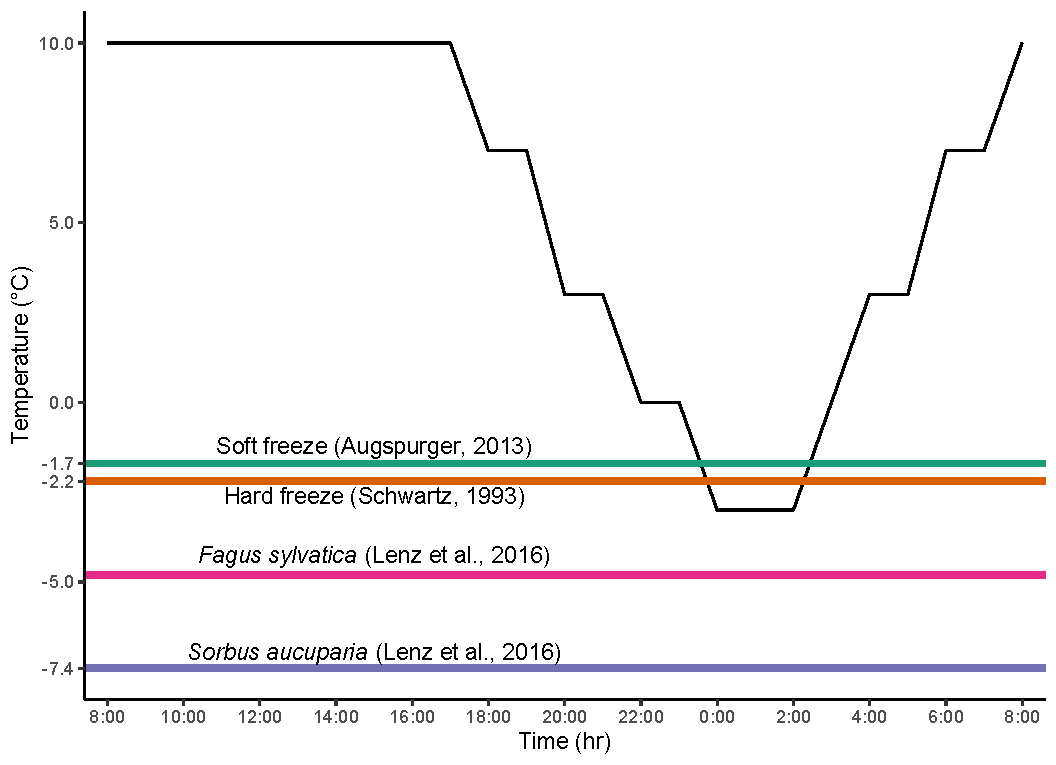
\includegraphics[width=12cm]{..//analyses/figures/growthchamber.pdf}
  -\caption{False spring treatment temperature regime in the growth chamber}\label{fig:gccond}
  -\end{center}
  -\end{figure}}
  
  {\begin{figure} [H]
  -\begin{center}
  -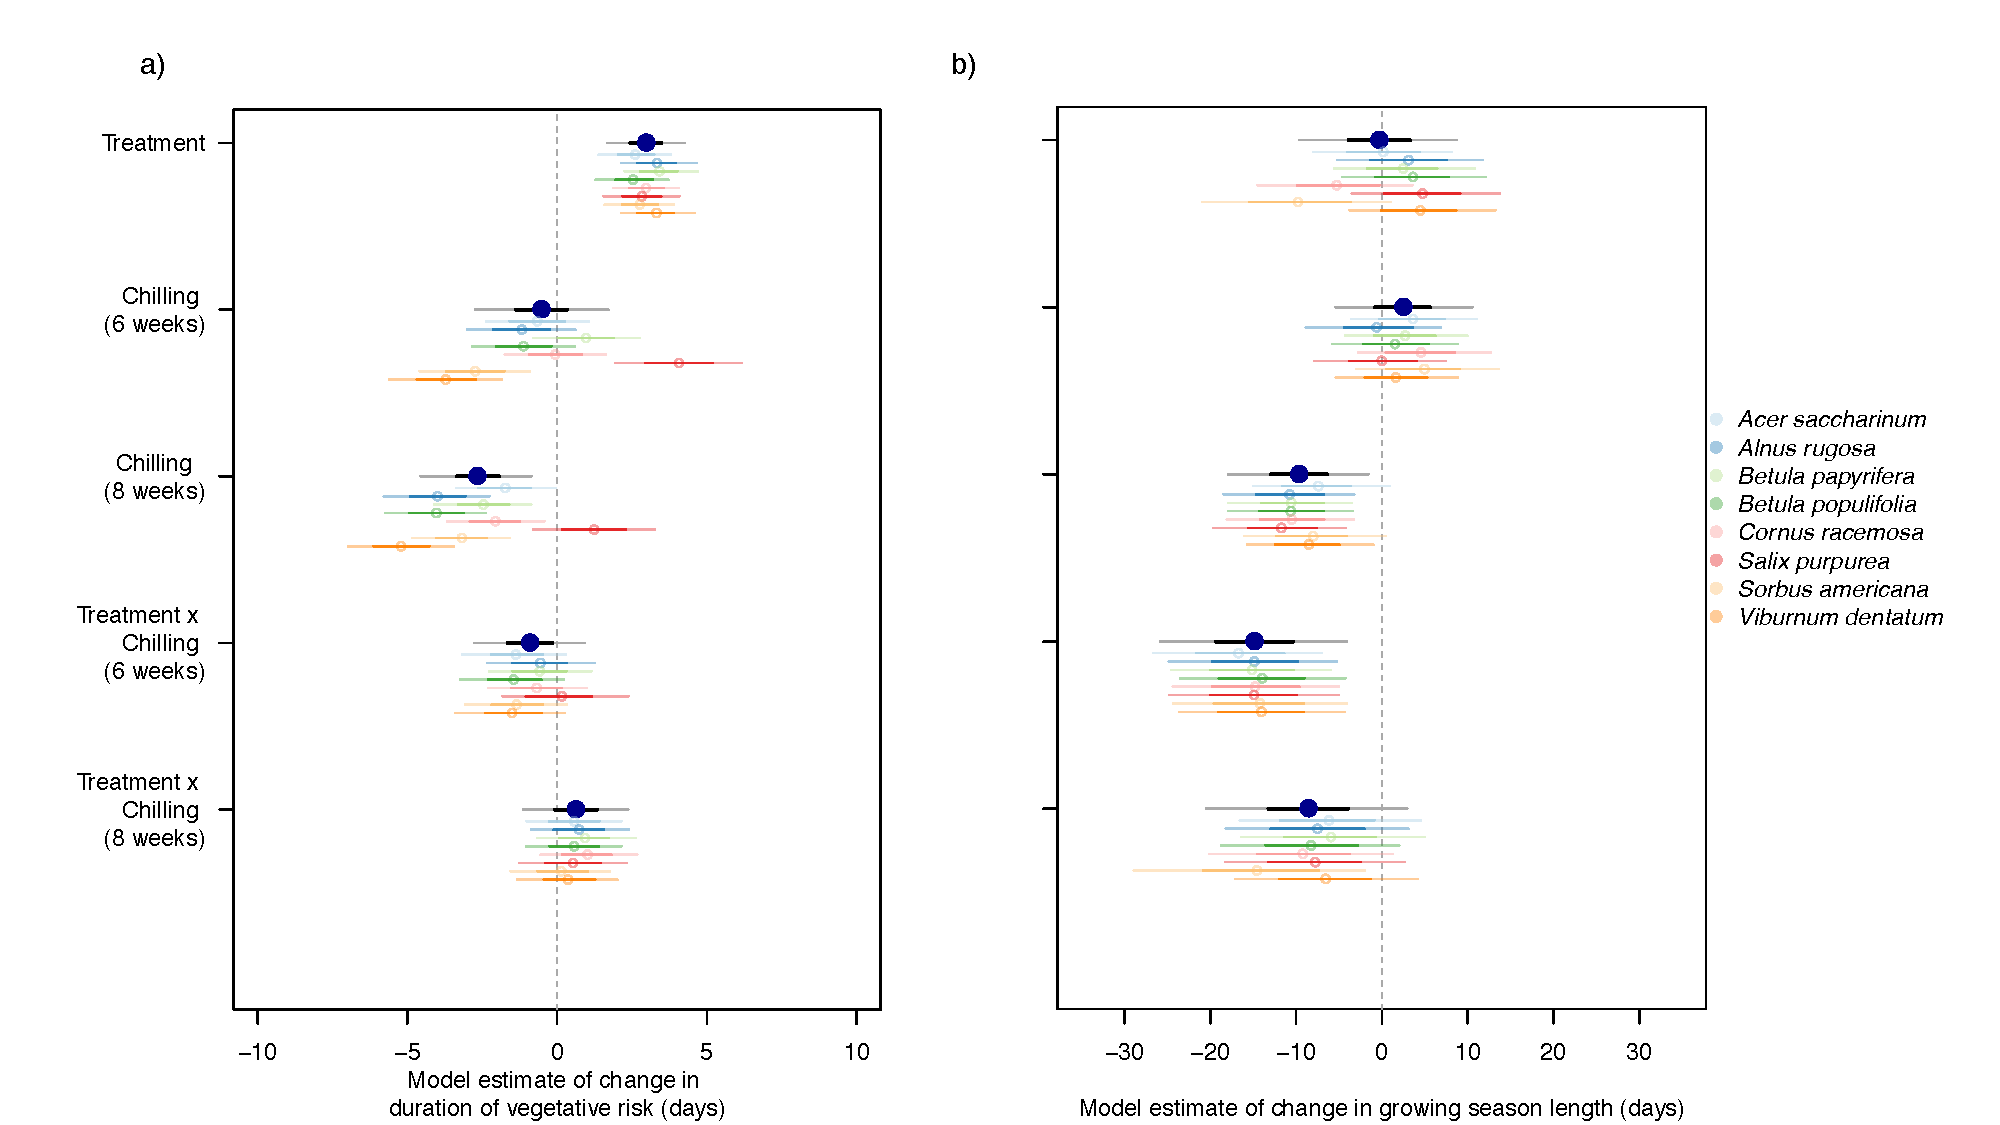
\includegraphics[width=18cm]{..//analyses/figures/mu_phen.pdf} 
  -\caption{Effects of false spring treatment, six weeks of chilling and eight weeks of chilling relative to four weeks of chilling with no false spring on a) duration of vegetative risk (days) and b) growing season length (days). Dots and thin lines show means and 90\% uncertainty intervals and thicker lines show 50\% uncertainty intervals. Larger blue dots represent overall estimates across all species, while smaller dots are estimates for each species. }\label{fig:muphen} 
  -\end{center}
  -\end{figure}}
  
  {\begin{figure} [H]
  -\begin{center}
  -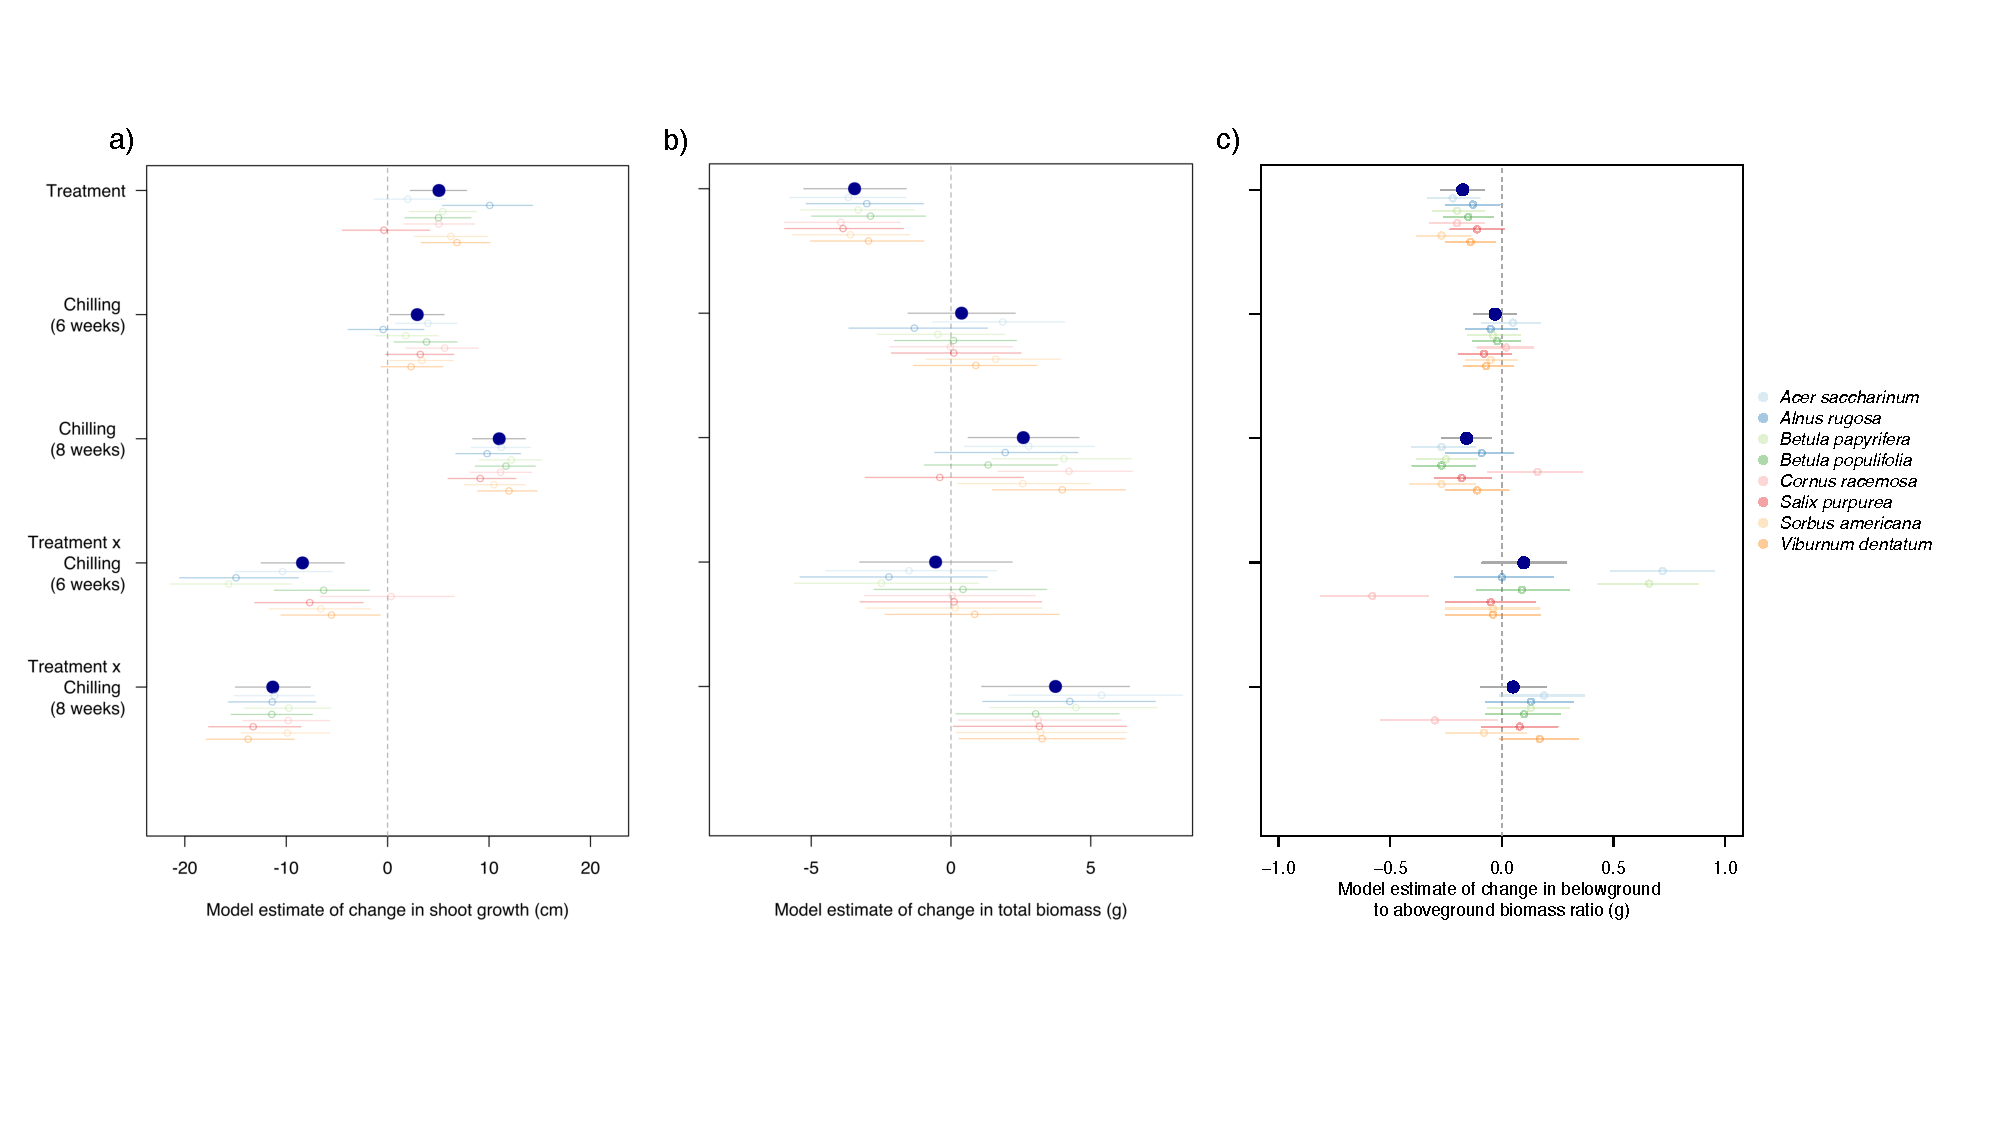
\includegraphics[width=18cm]{..//analyses/figures/mu_growth.pdf} 
  -\caption{Effects of false spring treatment, six weeks of chilling and eight weeks of chilling on a) shoot apical meristem damage and b) total shoot growth as a metric of height (cm). Dots and thin lines show means and 90\% uncertainty intervals and thicker lines show 50\% uncertainty intervals. Larger blue dots represent overall estimates across all species, while smaller dots are estimates for each species. }\label{fig:mugrowth}
  -\end{center}
  -\end{figure}}
  
  {\begin{figure} [H]
  -\begin{center}
  -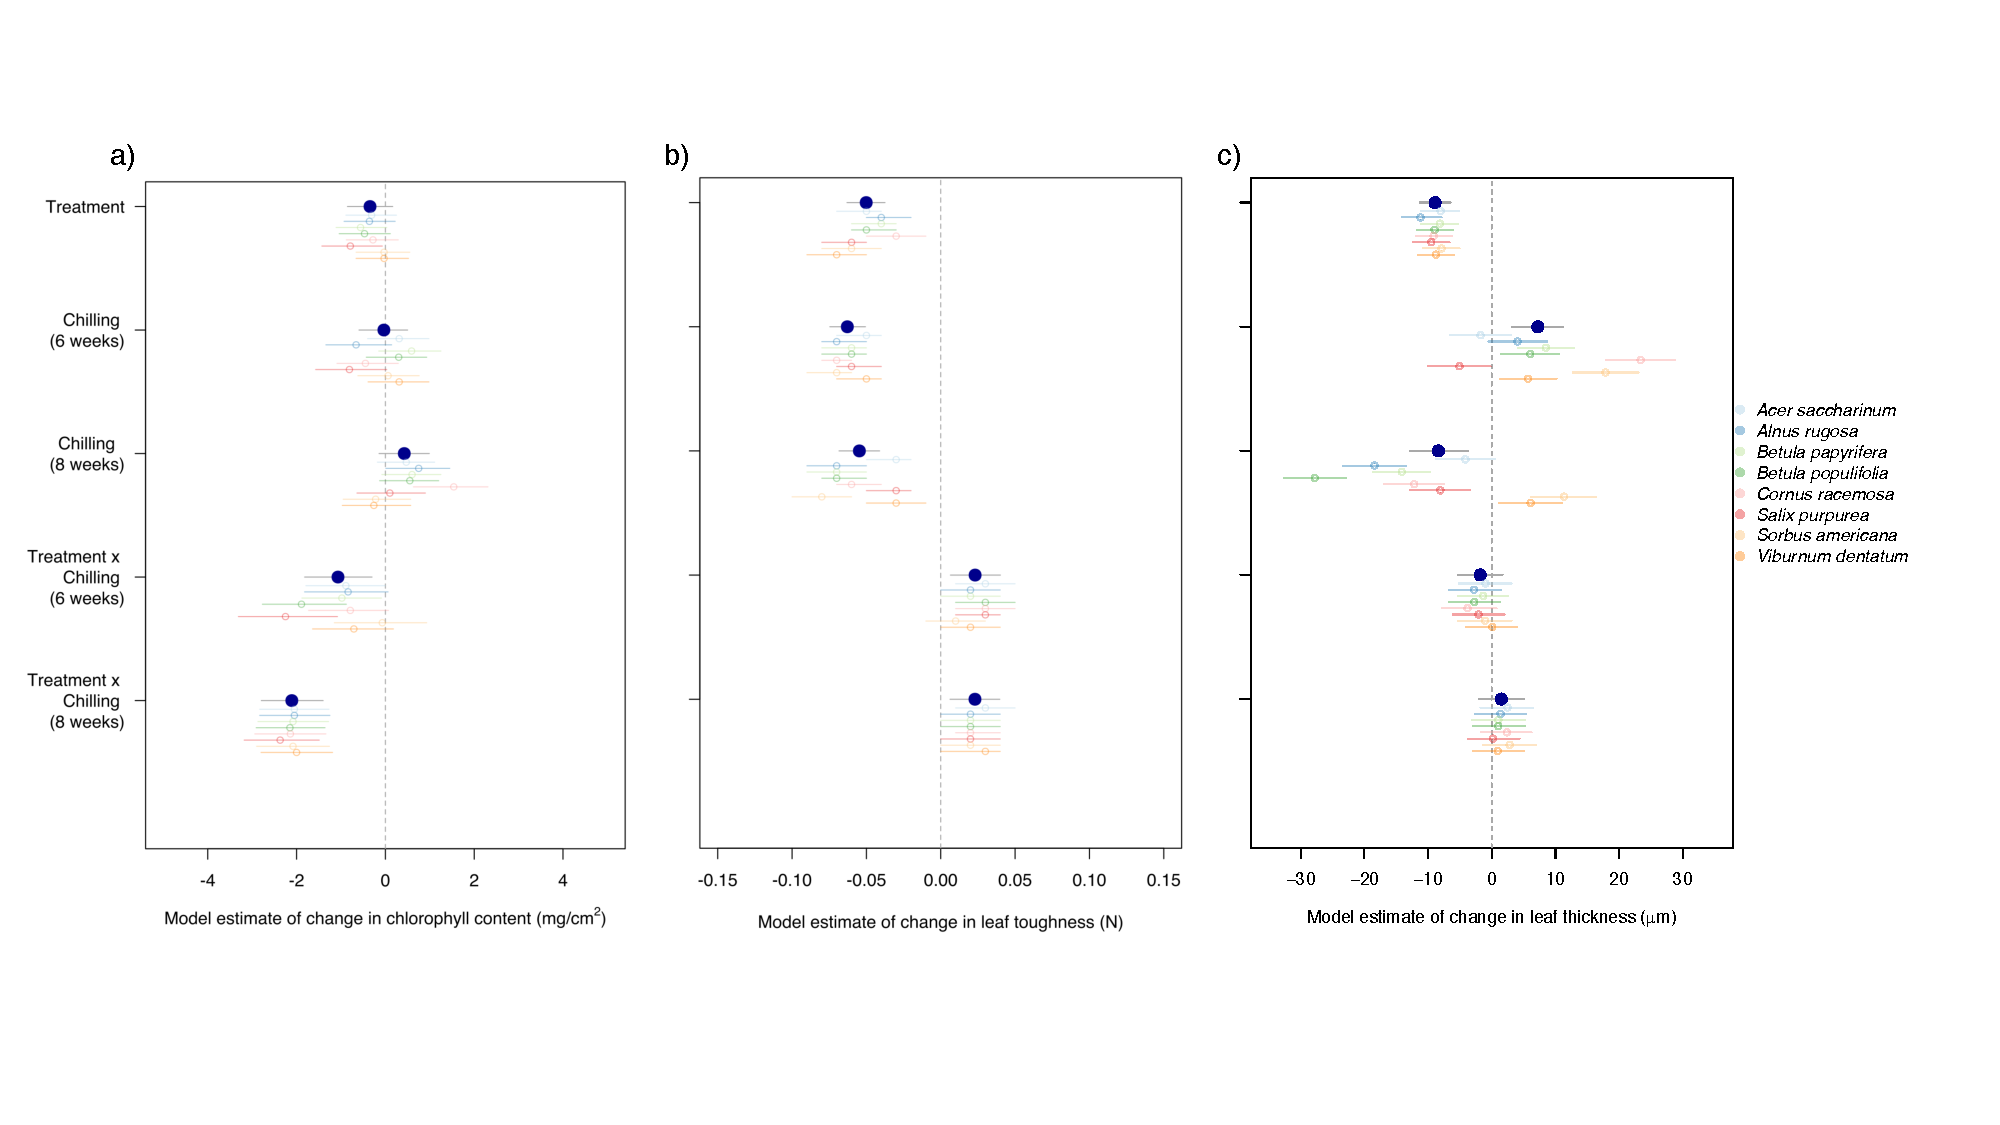
\includegraphics[width=18cm]{..//analyses/figures/mu_leaftraits.pdf} 
  -\caption{Effects of false spring treatment, six weeks of chilling and eight weeks of chilling on a) leaf toughness (N) and b) leaf thickness ($\mu$m). Dots and thin lines show means and 90\% uncertainty intervals and thicker lines show 50\% uncertainty intervals. Larger blue dots represent overall estimates across all species, while smaller dots are estimates for each species. }\label{fig:muleaf}
  -\end{center}
  -\end{figure}}
  
  {\begin{figure} [H]
  -\begin{center}
  -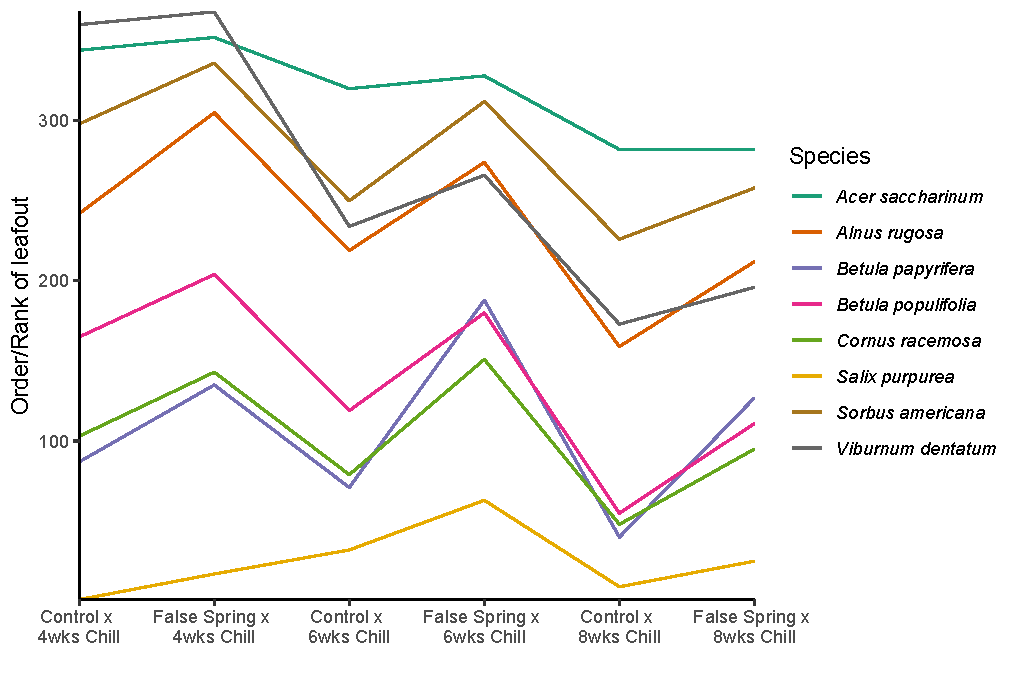
\includegraphics[width=12cm]{..//analyses/figures/leafoutorder_byrank.pdf} 
  -\caption{Rank order of leafout across all species using mean trends. }\label{fig:rank}
  -\end{center}
  -\end{figure}}
  

\end{document}
